\documentclass[border=10pt]{standalone}
\usepackage[svgnames]{xcolor}
\usepackage{amsmath}
\usepackage{pgfplots}
\pgfplotsset{compat=newest}
\usepackage[sfdefault]{FiraSans}
\usepackage{FiraMono}
\renewcommand*\familydefault{\sfdefault}
\begin{document}
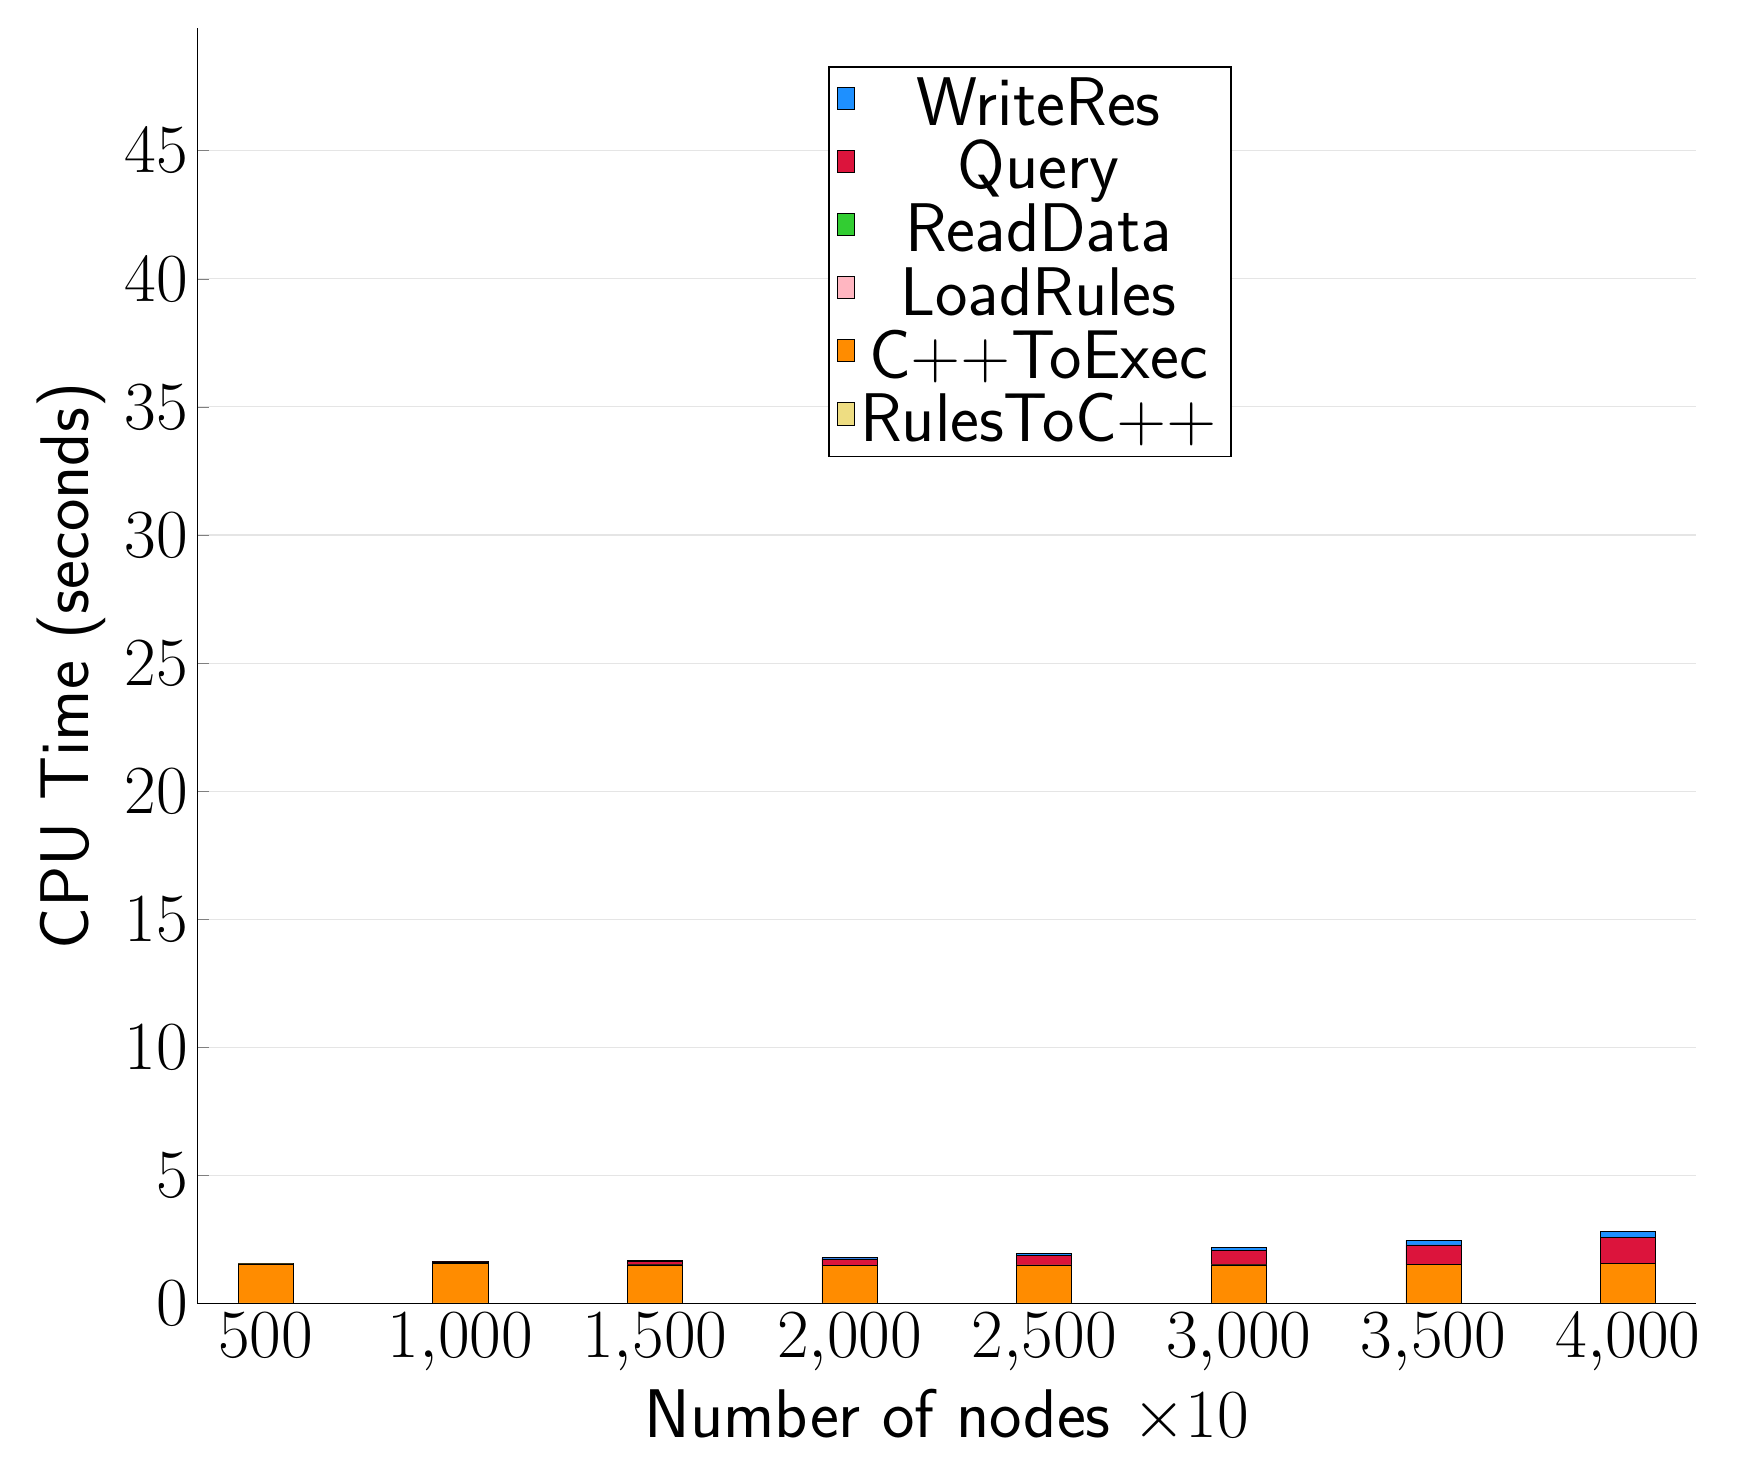
\begin{tikzpicture}
	\begin{axis}[
			ybar stacked,
			width=1.7\textwidth,
			bar width=0.7cm,
			ymajorgrids, tick align=inside,
			major grid style={draw=gray!20},
			xtick=data,
			ymin=0, ymax=49.78293,
			axis x line*=bottom,
			axis y line*=left,
			enlarge x limits=0.05,
			legend style={
					at={(0.69, 0.97)},
					anchor=north east,
					legend columns=1,
					font=\Huge,
				},
			ylabel={CPU Time (seconds)},
			xlabel={Number of nodes $\times 10$},
			label style={font=\Huge},
			tick label style={font=\Huge},
		]
		\addlegendimage{fill=DodgerBlue, draw=black, line width=0.2pt}
		\addlegendentry{WriteRes}
		\addlegendimage{fill=Crimson, draw=black, line width=0.2pt}
		\addlegendentry{Query}
		\addlegendimage{fill=LimeGreen, draw=black, line width=0.2pt}
		\addlegendentry{ReadData}
		\addlegendimage{fill=LightPink, draw=black, line width=0.2pt}
		\addlegendentry{LoadRules}
		\addlegendimage{fill=DarkOrange, draw=black, line width=0.2pt}
		\addlegendentry{C++ToExec}
		\addlegendimage{fill=LightGoldenrod, draw=black, line width=0.2pt}
		\addlegendentry{RulesToC++}
		\addplot +[fill=LightGoldenrod, draw=black, line width=0.2pt] coordinates {
				(500, 0.030000000000000006)
				(1000, 0.030000000000000006)
				(1500, 0.030000000000000006)
				(2000, 0.030000000000000006)
				(2500, 0.030000000000000006)
				(3000, 0.030000000000000006)
				(3500, 0.030000000000000006)
				(4000, 0.030000000000000006)
			};
		\addplot +[fill=DarkOrange, draw=black, line width=0.2pt] coordinates {
				(500, 1.522)
				(1000, 1.5400000000000003)
				(1500, 1.4850000000000003)
				(2000, 1.4700000000000002)
				(2500, 1.473)
				(3000, 1.483)
				(3500, 1.4889999999999999)
				(4000, 1.525)
			};
		\addplot +[fill=LightPink, draw=black, line width=0.2pt] coordinates {
				(500, 8.209999999999999e-05)
				(1000, 7.439999999999999e-05)
				(1500, 0.00010890000000000002)
				(2000, 0.00010740000000000001)
				(2500, 0.00011150000000000001)
				(3000, 9.92e-05)
				(3500, 8.58e-05)
				(4000, 0.00010250000000000001)
			};
		\addplot +[fill=LimeGreen, draw=black, line width=0.2pt] coordinates {
				(500, 0.0011086)
				(1000, 0.0019181000000000003)
				(1500, 0.0035159999999999996)
				(2000, 0.004493200000000001)
				(2500, 0.005503900000000001)
				(3000, 0.006535400000000001)
				(3500, 0.007031999999999999)
				(4000, 0.0080124)
			};
		\addplot +[fill=Crimson, draw=black, line width=0.2pt] coordinates {
				(500, 0.0148894)
				(1000, 0.058338999999999995)
				(1500, 0.13507059999999999)
				(2000, 0.23820510000000006)
				(2500, 0.37549179999999993)
				(3000, 0.5541748)
				(3500, 0.7649524000000001)
				(4000, 1.018127)
			};
		\addplot +[fill=DodgerBlue, draw=black, line width=0.2pt] coordinates {
				(500, 0.004368199999999999)
				(1000, 0.014265799999999999)
				(1500, 0.031566500000000004)
				(2000, 0.0564145)
				(2500, 0.08798500000000001)
				(3000, 0.1261758)
				(3500, 0.17266189999999998)
				(4000, 0.22527880000000003)
			};
	\end{axis}
\end{tikzpicture}

\end{document}
